We conducted over 20 experimental setups, with each one consisting of five independent runs with different seeds. In this chapter, a subset of the results is displayed and the systematic approach of finding suitable hyperparameters and the interpretation about their influence is described. A table of all results can be found in the appendix in section \ref{appendix:curveResults}.
\par
Let us start by recalling what components are present and whether they are immutable during our experiments. Foremost, there are five different state representations and their corresponding action spaces as the simplest environment in the case of $S1$ and $S2$ adjusts the speed automatically. The combinations to test are thus $S1\_A1$, $S2\_A1$, $S3\_A2$, $S4\_A2$ and $S5\_A2$.
\par
Next are the hyperparameters as described in \ref{subchap:hyperparameters}. We will keep the values of the parameters unchanged during the experiments except for the replay buffer size and $\sigma$, which has a huge influence on the exploration due to its impact on the noise process (see Fig. \ref{fig:ouProcess}). We adjust the source code of the Stable-Baselines3 library to support different learning rates for the actor and critic networks to stay in line with the theoretical findings of chapter \ref{subchap:hyperparameters}. Hence, we use a fixed learning rate of $10^{-4}$ for the actor and  $10^{-3}$ for the critic. The training lasts for a fixed duration of 30,000 time steps, which translates to almost identical numbers of network updates (during the initial filling of the replay buffer no updates are done) and 492 episodes. We described the neuronal network architecture by using the notion $n_h^i= N$, where $n$ is the $i$-th hidden layers, starting at 1, with $N$ neurons. The hyperparameters are summarized as follows:

\begin{table}[H]
\centering
\begin{tabular}{|l|l|}
\hline
\textbf{Name}                & \textbf{Value}                                                \\ \hline
Training Steps               & $30.000$                                                      \\ \hline
Network Architecture         & $n_{h}^{1}=400$ and $n_{h}^{2}=300$       \\ \hline
Learning Rates               & $\alpha_{actor} = 10^{-4}$ and $\alpha_{critic}= 10^{-3}$     \\ \hline
Batch Size                   & $128$                                                         \\ \hline
Soft Update Parameter $\tau$ & $10^{-3}$                                                     \\ \hline
Discount Factor $\gamma$     & $0.99$                                                        \\ \hline
Replay Buffer Size           & $5\cdot 10^4$ or $5 \cdot 10^6$                               \\ \hline
Noise Parameter              & $\mu=0$, $\theta=0.15$, $\sigma$ is $0.05$ or $0.15$ or $0.5$ \\ \hline
\end{tabular}
\caption{\label{tab:hyperDDPG} Hyperparameter setup during DDPG training of the synthetic experiments}
\end{table}
\par
Lastly, investigations are done on the effect of the three different reward function ($R1$, $R2$ and $R3$) as defined in subchapter \ref{subchap:reward}.
\par
As a starting point, we interpret the results of the first sets of experiments, conducted with $\sigma=0.05$ and a replay buffer size of $N=5 \cdot 10^4$. A small value of $\sigma$ translates to overall smaller amplitudes in the Ornstein-Uhlenbeck process, which causes the noise to be added to suggested actions to alternate between $-0.5$ and $0.5$ as illustrated in Fig. \ref{fig:lowSigmaNoise}. The intention behind a low $\sigma$ value is related to the small replay buffer size because we do not want to fill up the buffer majorly with extreme action values close to or clipped at $-1$ and $1$. The upcoming table shows the performances (euclidean distances) and standard deviations of the best-seed runs and the respective euclidean distances of the agent's suggested and the ground-truth curves.

% Please add the following required packages to your document preamble:
% \usepackage[table,xcdraw]{xcolor}
% If you use beamer only pass "xcolor=table" option, i.e. \documentclass[xcolor=table]{beamer}
\begin{table}[H]
\centering
\begin{tabular}{|l|l|l|l|l|}
\hline
\multicolumn{1}{|c|}{\textbf{Experiment}} & \multicolumn{1}{c|}{\textbf{Overall Performance}} & \multicolumn{1}{c|}{\textbf{Curve\_A}} & \multicolumn{1}{c|}{\textbf{Curve\_B}} & \multicolumn{1}{c|}{\textbf{Curve\_C}} \\ \hline
$S1\_A1\_R1$                              & $207 \pm 180$                                     & $183$                                  & $319$                                  & $141$                                  \\ \hline
$S1\_A1\_R3$                              & $134 \pm 149$                                     & $130$                                  & $198$                                  & $87$                                   \\ \hline
$S2\_A1\_R1$                              & $141 \pm 122$                                     & $180$                                  & $156$                                  & $91$                                   \\ \hline
$S2\_A1\_R3$                              & $132 \pm 148$                                     & $112$                                  & $194$                                  & $101$                                  \\ \hline
$S3\_A2\_R1$                              & $165 \pm 158$                                     & $117$                                  & $312$                                  & $93$                                   \\ \hline
$S3\_A2\_R2$                              & $173 \pm 127$                                     & $195$                                  & $211$                                  & $121$                                  \\ \hline
$S3\_A2\_R3$                              & $154 \pm 116$                                     & $144$                                  & $116$                                  & $195$                                  \\ \hline
$S4\_A2\_R1$                              & $112 \pm 123$                                     & $117$                                  & $87$                                   & $128$                                  \\ \hline
{\color[HTML]{333333} $S4\_A2\_R2$}       & {\color[HTML]{333333} $91 \pm 98$}                & {\color[HTML]{333333} $56$}            & {\color[HTML]{333333} $134$}           & {\color[HTML]{333333} $90$}            \\ \hline
$S4\_A2\_R3$                              & $80 \pm 88$                                     & $71$                                  & $49$                                  & $112$                                  \\ \hline
$S5\_A2\_R1$                              & $199 \pm 118$                                     & $195$                                  & $204$                                  & $197$                                  \\ \hline
$S5\_A2\_R2$                              & $219 \pm 115$                                     & $238$                                  & $238$                                  & $185$                                  \\ \hline
\end{tabular}
\caption{ Performances of several experiments with $\sigma = 0.05$ and replay buffer size of $N=5 \cdot 10^4$.}
\label{tab:resultsK3}
\end{table}

To understand what these numbers really mean, we have to dive into deeper analysis and have to visualize actual trajectories produced by the agent. We first concentrate on the simplest environment variant, which does not require the agent to choose a speed value ($S1\_A1$ and $S2\_A1$). One assumption is that the state representation of $S1$ is insufficient due to the fact that the agent has no way to identify unique states of different curves if only $x$ and $y$ are given. However, the performances of $S1\_A1\_R3$ and $S2\_A2\_R3$ are almost identical. The question arises if this proves that the assumption is wrong or the agent fails the task catastrophically in both cases? To answer this question, we visualize both runs in a way to quantify the evolving distances during each of the three different episodes:
\par

\begin{figure}[H]
     \centering
     \begin{subfigure}[b]{0.9\textwidth}
         \centering
         \includesvg[width=\textwidth]{images/ddpg_results/simple_envs_S1_S2/ddpg_S1_A1_R3_K3.svg}
         \caption{$S1\_A1\_R3$}
     \end{subfigure}
\end{figure}
\begin{figure}[H]\ContinuedFloat
     \begin{subfigure}[b]{0.9\textwidth}
         \centering
         \includesvg[width=\textwidth]{images/ddpg_results/simple_envs_S1_S2/ddpg_S2_A1_R3_K3.svg}
         \caption{$S2\_A1\_R3$}
     \end{subfigure}
        \caption{Distances between the path proposed by the agent and the GT over time. $\sigma = 0.15$ and $N=5\cdot 10^4$.}
        \label{fig:simpleCurves1}
\end{figure}

Fig. \ref{fig:simpleCurves1} displays the inability of both state representations to follow and reproduce $curve\_B$ as both setups drift apart from the GT right at the beginning, reaching a distance from over 200 just 20 time steps into the episode. However, we do see similar mediocre performances in terms of the $curve\_A$ and $curve\_B$, with $S2$ following $curve\_A$ exceptional well in the mid-part of the episode between time steps 15 to 23. To analyze the behavior of the agent on an empirical level, we also visualize the generated trajectories by the agent. Please note, that the performance metric includes a  time component and the portrayal of the paths could lead to misinterpretation, for example, if the agent follows the path perfectly but on a slower pace. Nevertheless, those illustrations greatly help to analyze the behavior of the agent and algorithm. 

\begin{figure}[H]
     \centering
     \begin{subfigure}[b]{0.31\textwidth}
         \centering
         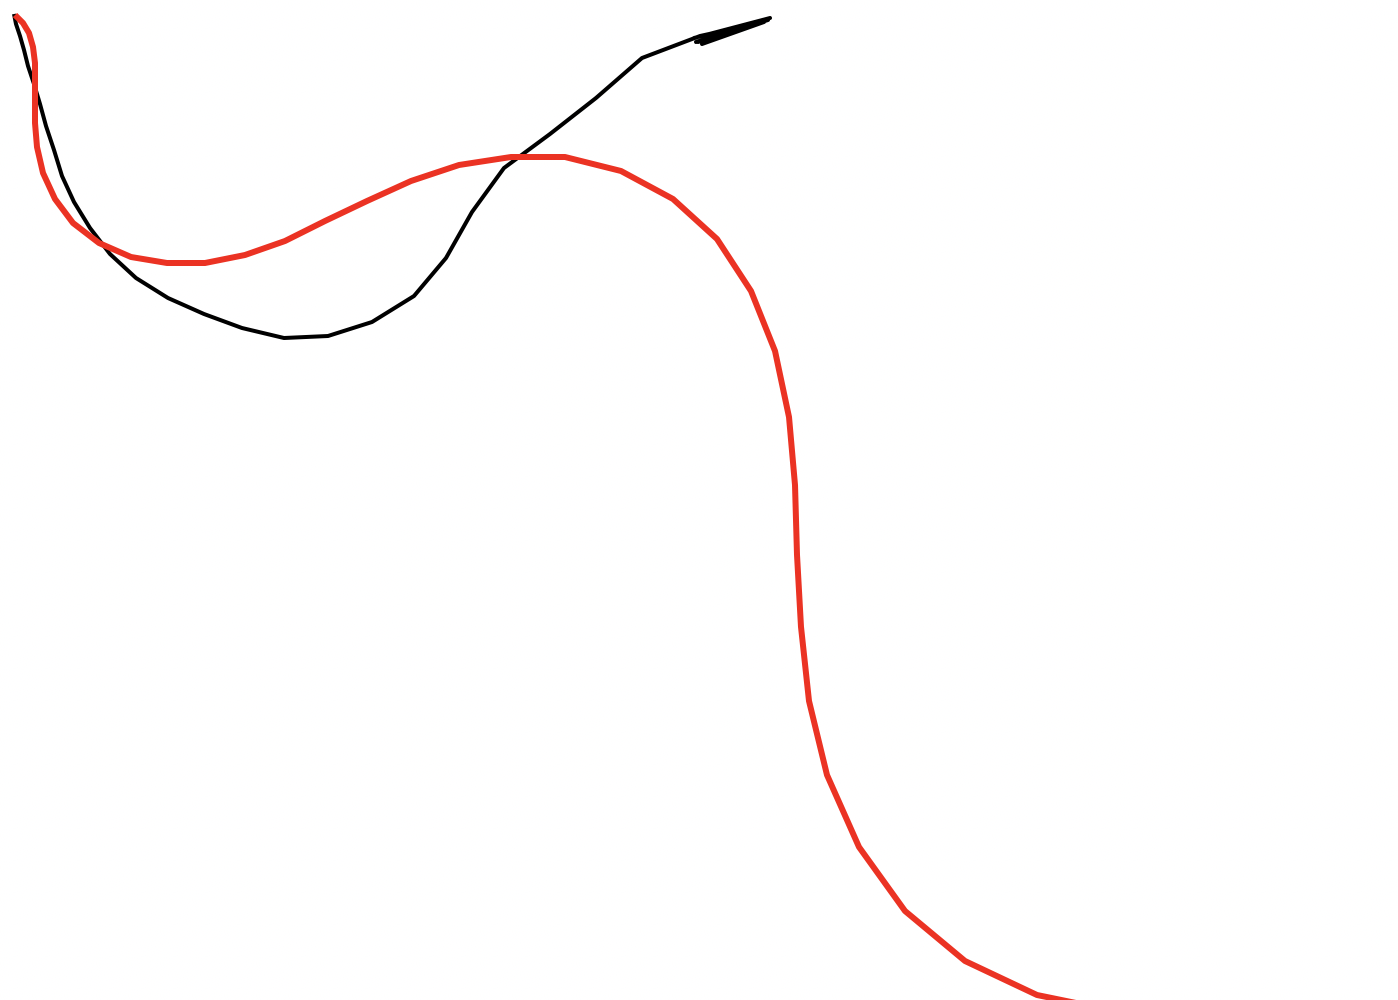
\includegraphics[width=\textwidth]{images/ddpg_results/simple_envs_S1_S2/S1_A1_R3_K3_curve_A.png}
         \caption{$curve\_A$}
     \end{subfigure}
     \hfill
     \begin{subfigure}[b]{0.31\textwidth}
         \centering
         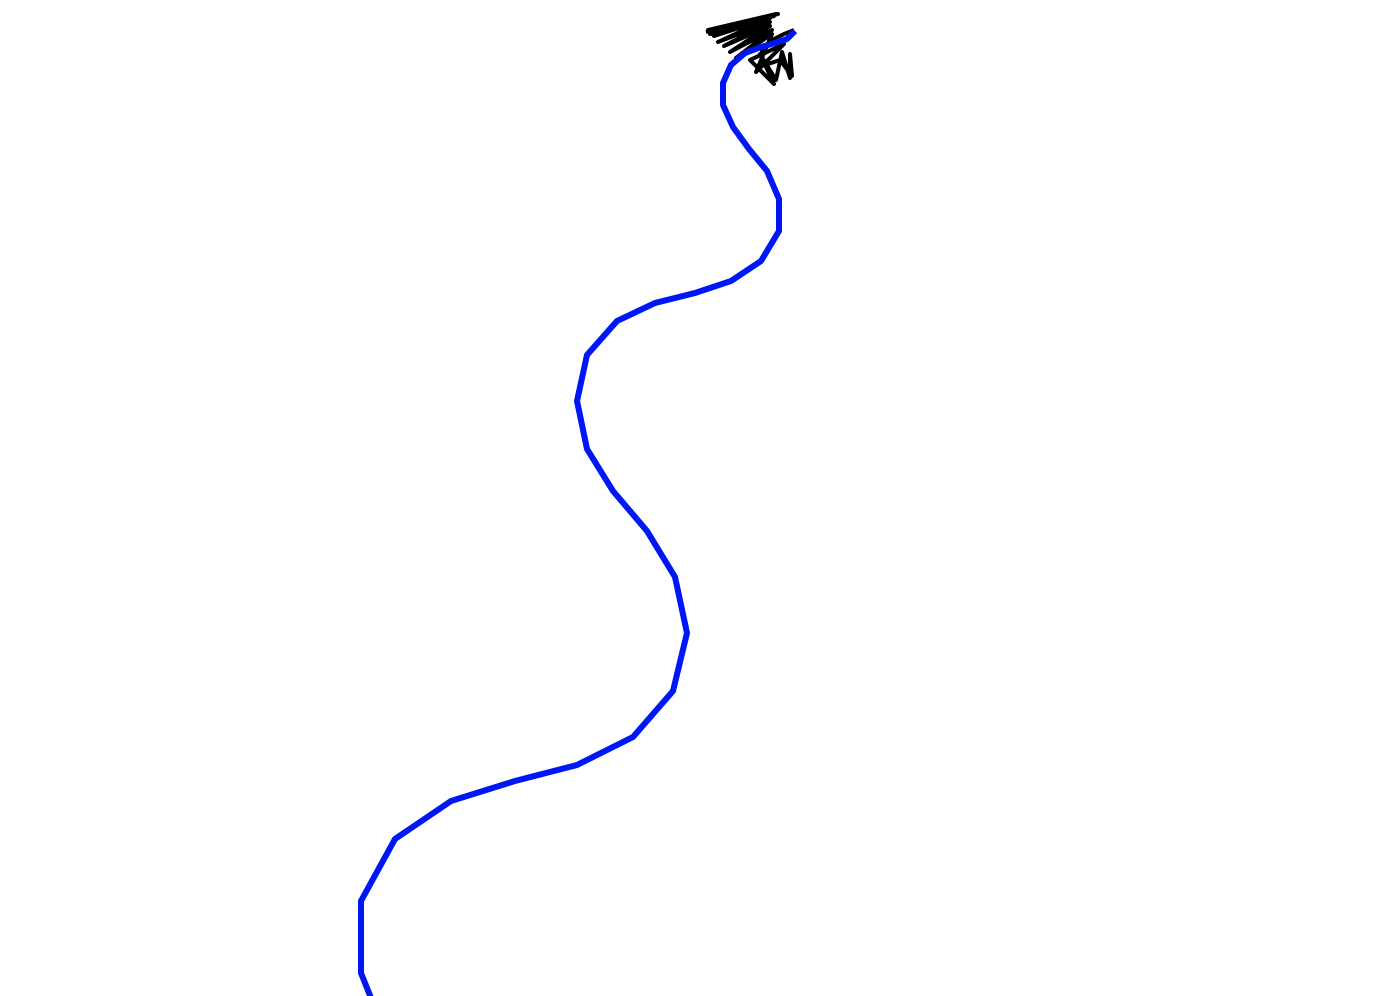
\includegraphics[width=\textwidth]{images/ddpg_results/simple_envs_S1_S2/S1_A1_R3_K3_curve_B.png}
         \caption{$curve\_B$}
     \end{subfigure}
     \hfill
     \begin{subfigure}[b]{0.31\textwidth}
         \centering
         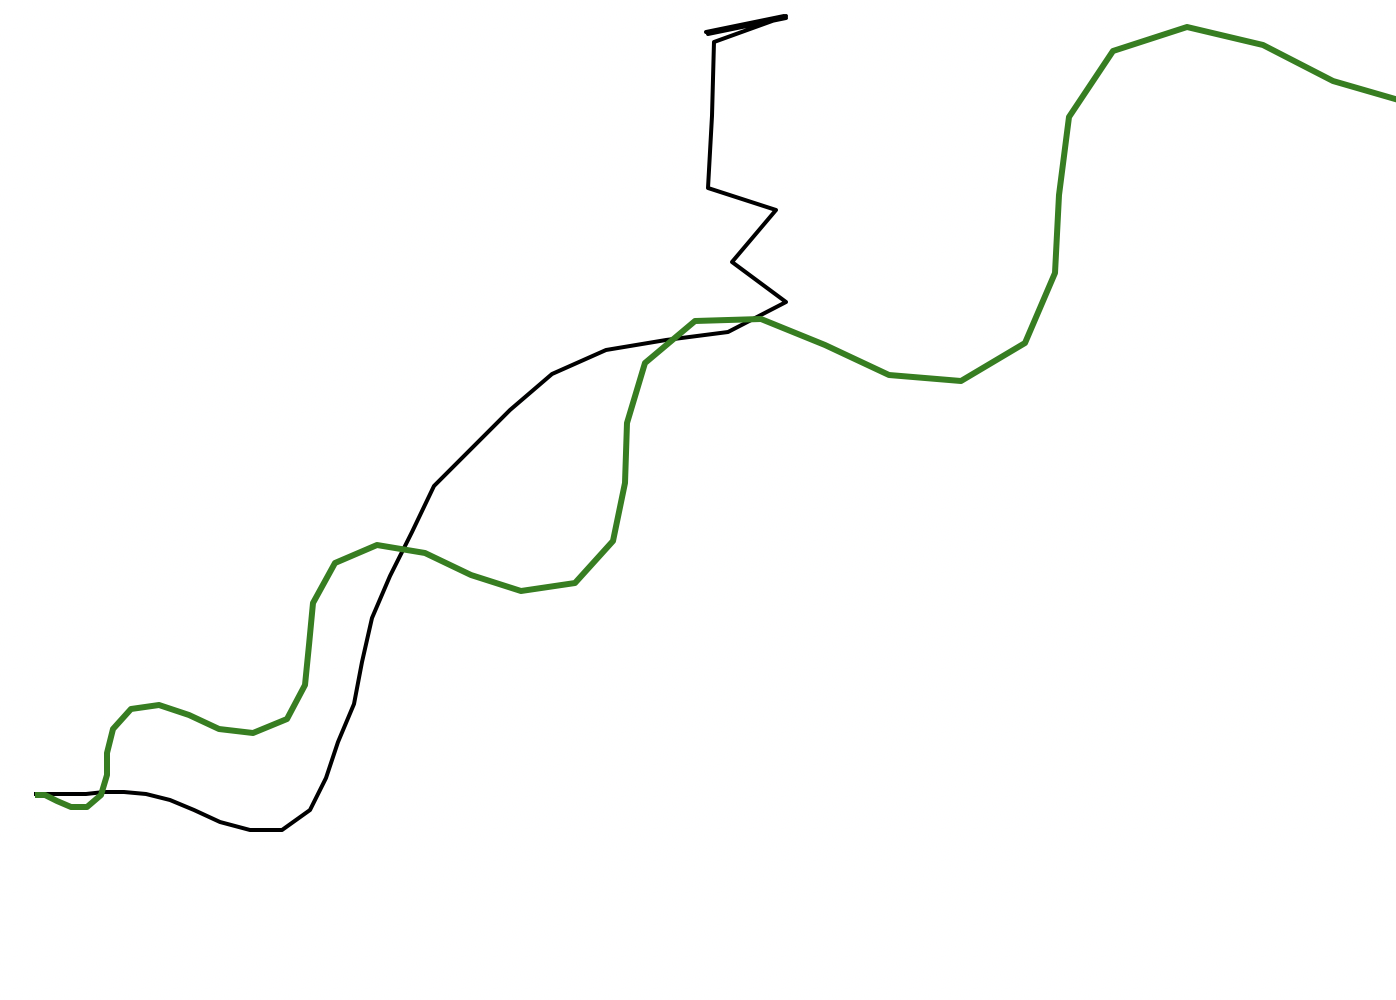
\includegraphics[width=\textwidth]{images/ddpg_results/simple_envs_S1_S2/S1_A1_R3_K3_curve_C.png}
         \caption{$curve\_C$}
     \end{subfigure}
        \caption{$S1\_A1\_R3$}
        \label{fig:simpleCurves2}
\end{figure}



\begin{figure}[H]
     \centering
     \begin{subfigure}[b]{0.31\textwidth}
         \centering
         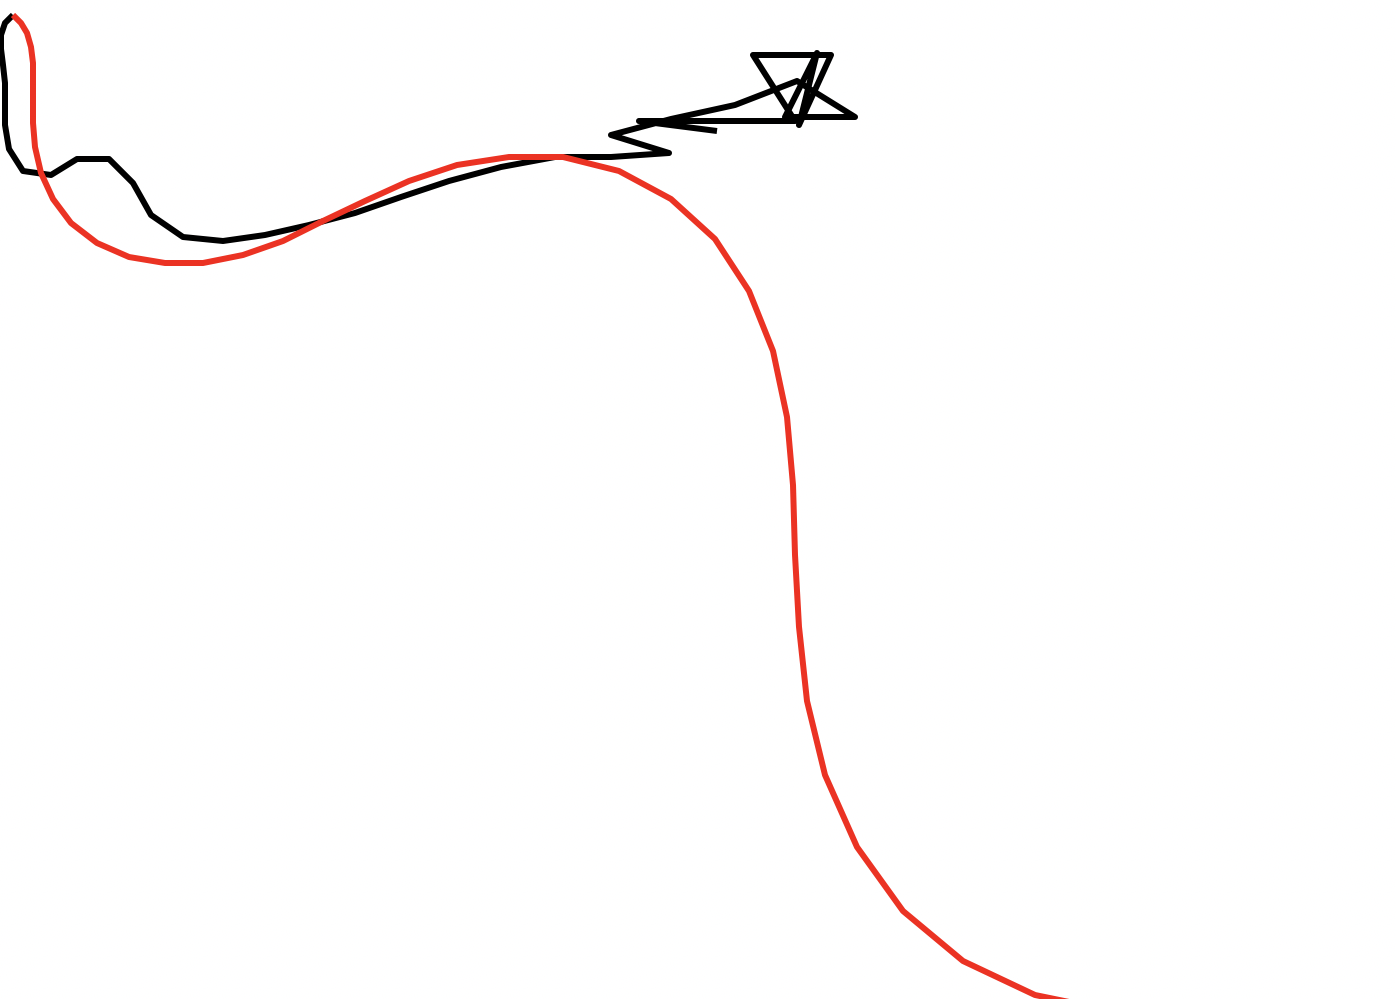
\includegraphics[width=\textwidth]{images/ddpg_results/simple_envs_S1_S2/S2_A1_R3_K3_curve_A.png}
         \caption{$curve\_A$}
     \end{subfigure}
     \hfill
     \begin{subfigure}[b]{0.31\textwidth}
         \centering
         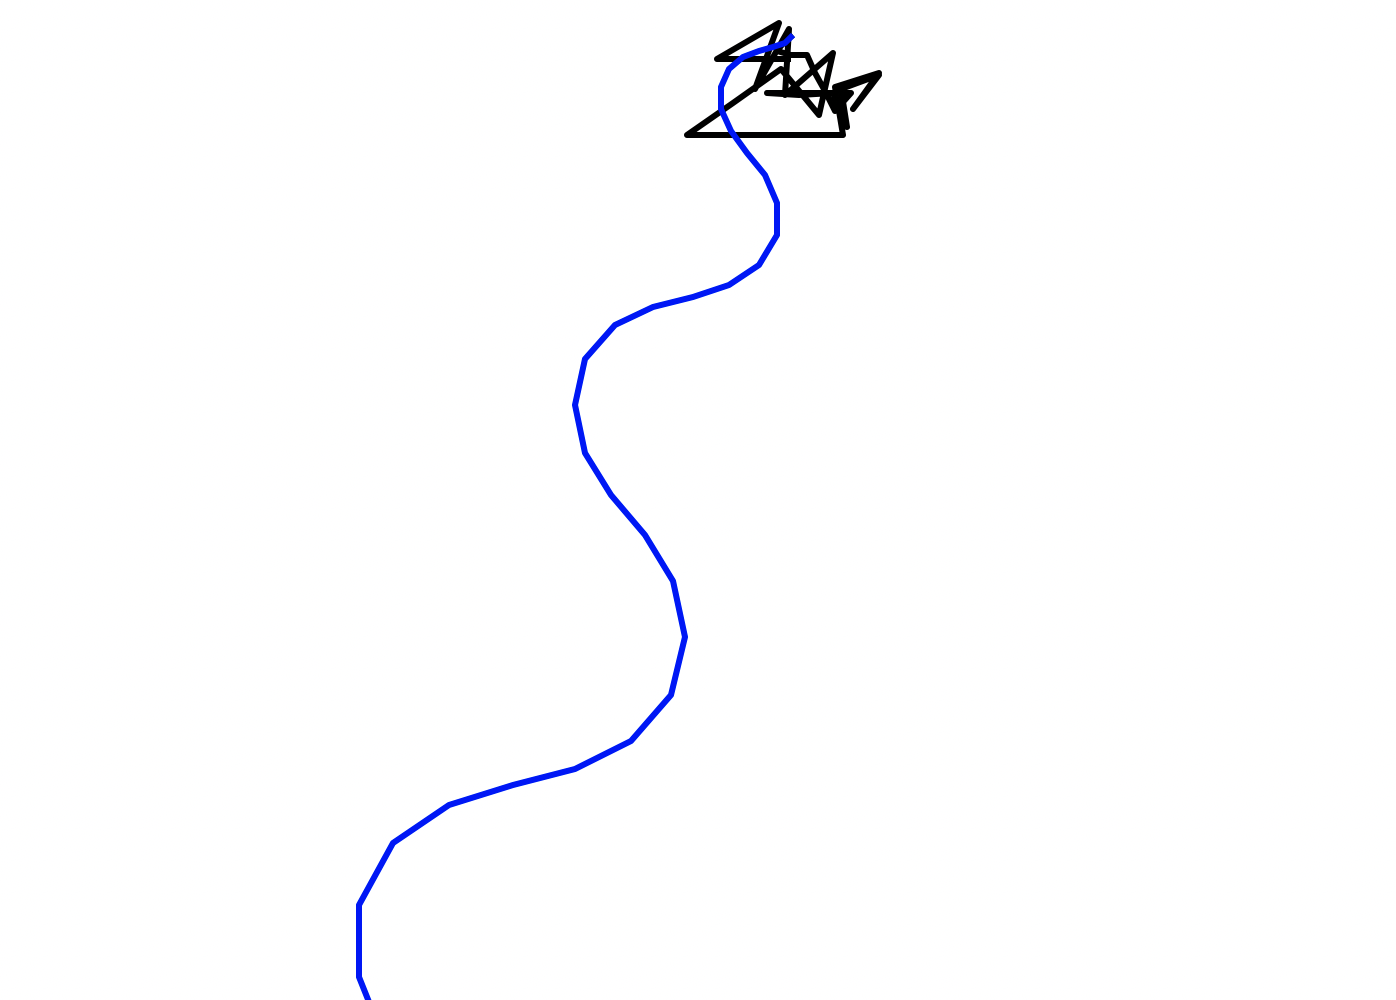
\includegraphics[width=\textwidth]{images/ddpg_results/simple_envs_S1_S2/S2_A1_R3_K3_curve_B.png}
         \caption{$curve\_B$}
     \end{subfigure}
     \hfill
     \begin{subfigure}[b]{0.31\textwidth}
         \centering
         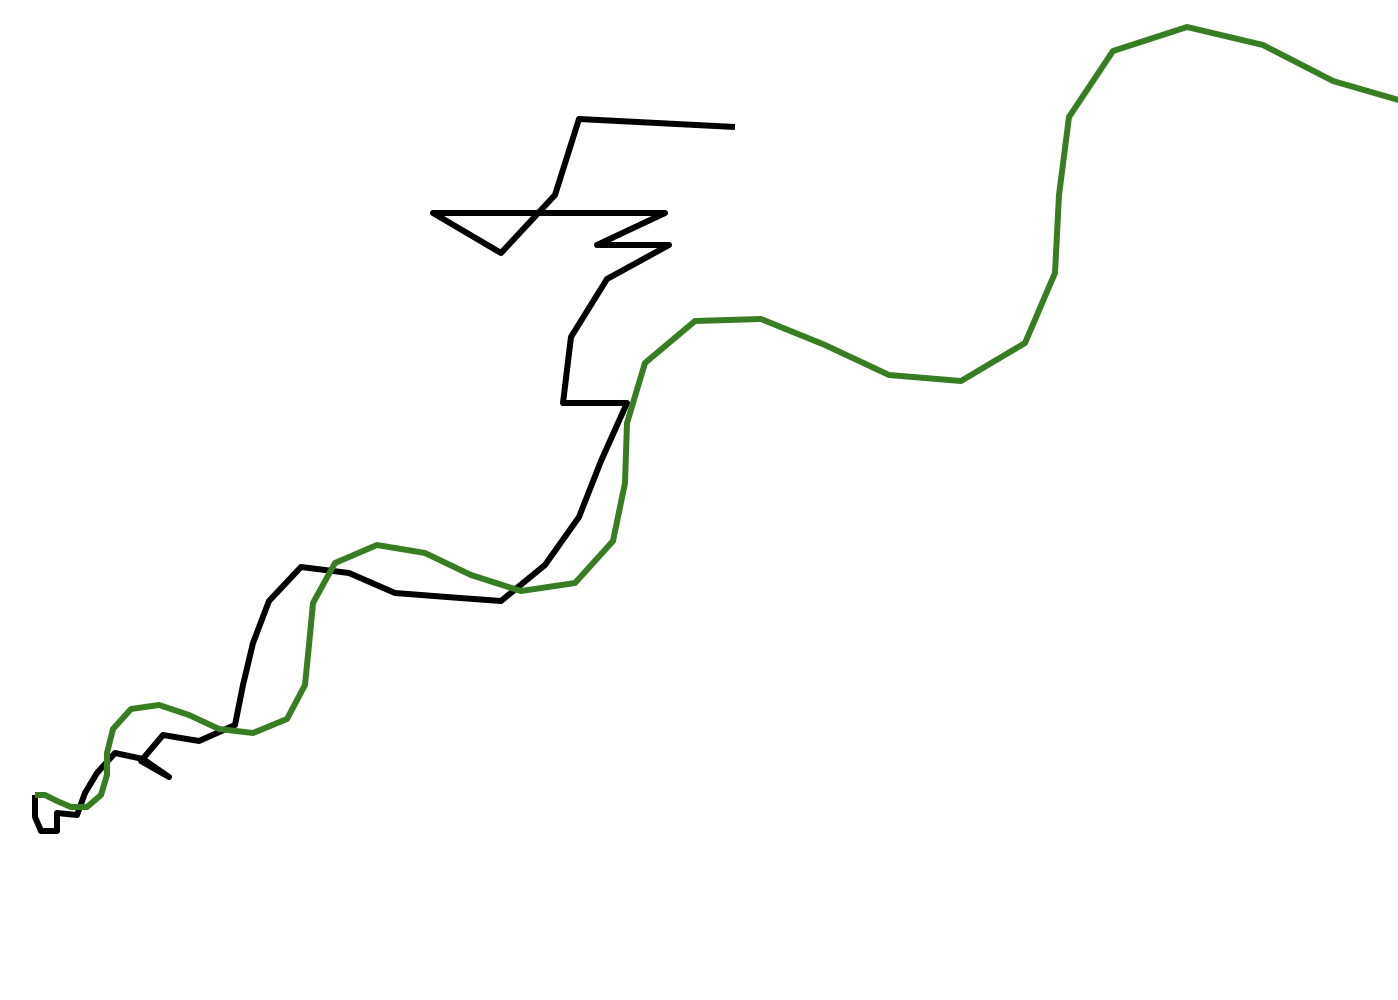
\includegraphics[width=\textwidth]{images/ddpg_results/simple_envs_S1_S2/S2_A1_R3_K3_curve_C.png}
         \caption{$curve\_C$}
     \end{subfigure}
        \caption{$S2\_A1\_R3$}
        \label{fig:simpleCurves3}
\end{figure}

The illustrations of Fig. \ref{fig:simpleCurves2} and \ref{fig:simpleCurves3} indeed reveal catastrophic failure to the task for both state representations. Although the starting time steps for $curve\_A$ and $curve\_C$ look promising, the agent suddenly drifts apart heavily from the GT path. It is noticeable that the agent, in all cases, moves towards a certain area to then start fluctuating the proposed heading value so much that it stays in the area. The area is located in the center top of the map where the blue $curve\_B$ has its starting position, which in returns explains the bad performance for this specific curve. 
\par
It is hard to reason exactly what is causing this behavior. One reason could be the $\sigma$ value being too low so that the agent is unable to explore the correct heading values for $curve\_B$, which eventually leads to randomly guessing values right at the beginning of the episode of $curve\_B$ and thus the filling of the replay buffer with bad transition tuples. Another possible explanation for this behavior could be that the replay buffer is too small, only fitting in $5\cdot 10^4$ transitions. Another indicator of this could be the general drift after approximately 25 time steps for $curve\_A$ and $curve\_C$ as the replay buffer is unable to contain the transition tuples for the complete paths.
\par
To test these hypotheses, we conduct another set of experiments with an increased value for $\sigma$ and a replay buffer size of $N=5\cdot 10^6$. The performances are $157 \pm 145$ in the case of $S1\_A1\_R3$ and $182 \pm 181$ for $S2\_A1\_R3$ which is even worse than the results of the previous setting display in Tab. \ref{tab:resultsK3}. The generated paths of the best run of $S2\_A1\_R3$ show that the agent now starts fluctuating on place for $curve\_C$ as well:

\begin{figure}[H]
     \centering
     \begin{subfigure}[b]{0.31\textwidth}
         \centering
         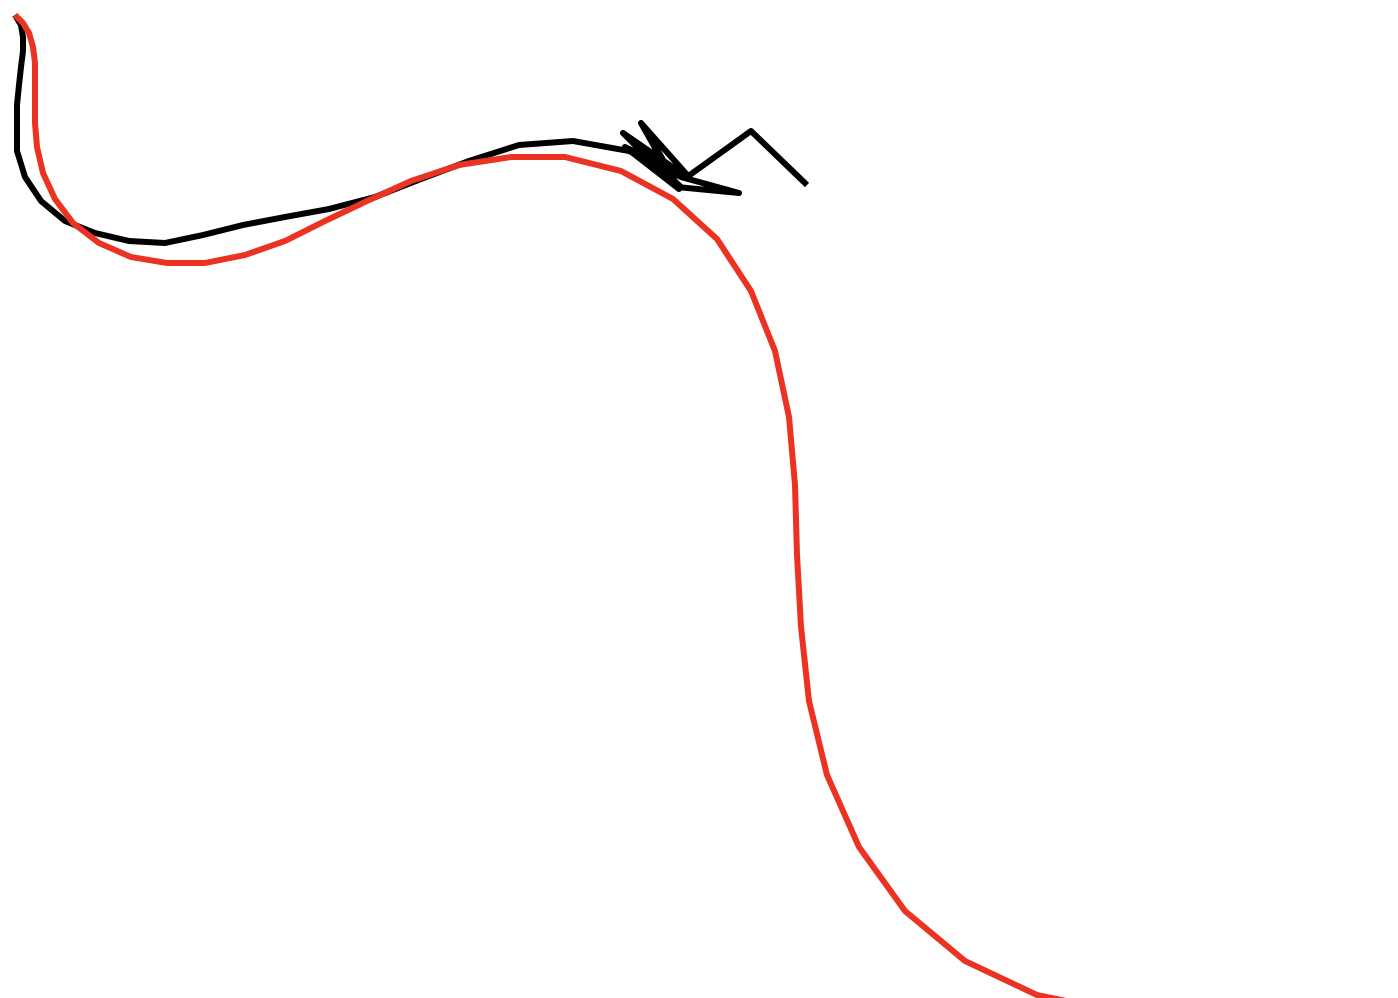
\includegraphics[width=\textwidth]{images/ddpg_results/simple_envs_S1_S2/S2_A1_R3_5mio_curve_A.png}
         \caption{$curve\_A$}
     \end{subfigure}
     \hfill
     \begin{subfigure}[b]{0.31\textwidth}
         \centering
         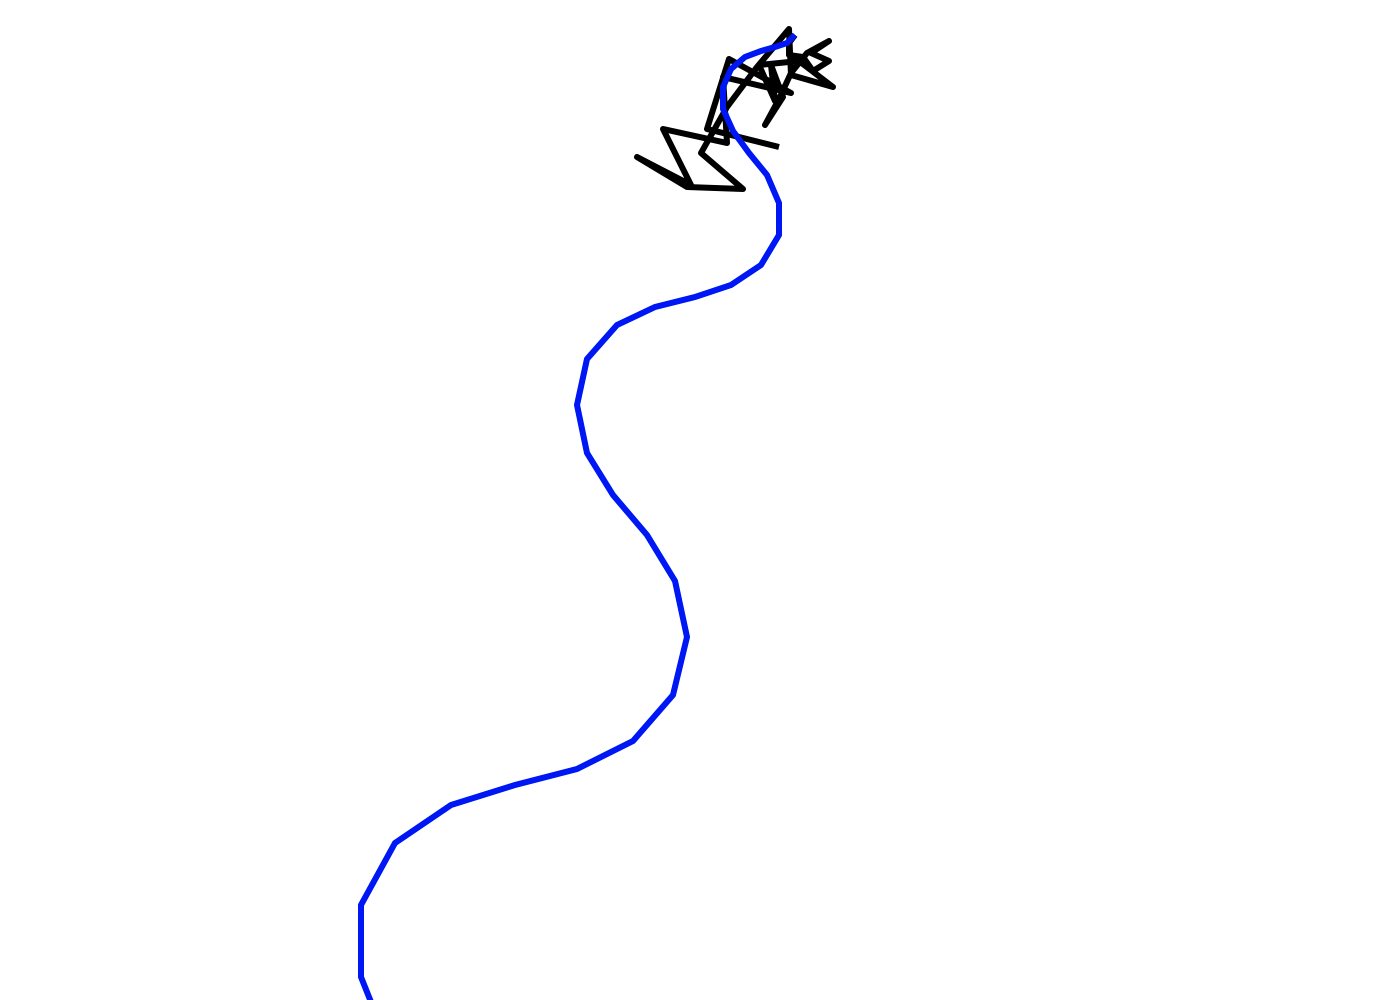
\includegraphics[width=\textwidth]{images/ddpg_results/simple_envs_S1_S2/S2_A1_R3_5mio_curve_B.png}
         \caption{$curve\_B$}
     \end{subfigure}
     \hfill
     \begin{subfigure}[b]{0.31\textwidth}
         \centering
         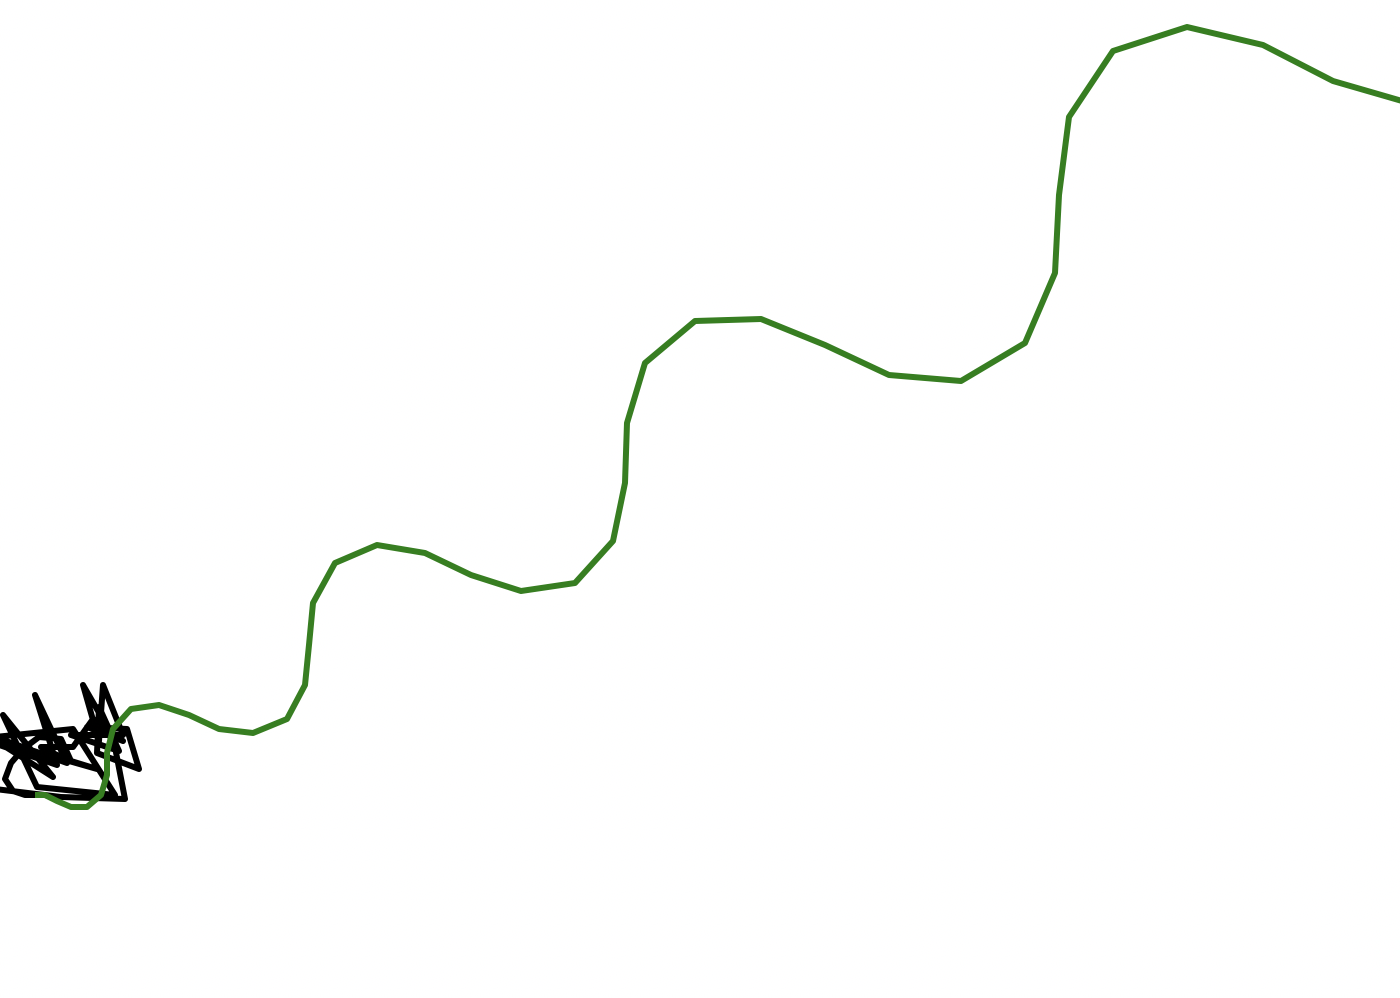
\includegraphics[width=\textwidth]{images/ddpg_results/simple_envs_S1_S2/S2_A1_R3_5mio_curve_C.png}
         \caption{$curve\_C$}
     \end{subfigure}
        \caption{$2\_A1\_R3$ using $\sigma=0.15$ and a replay buffer size of $N=5\cdot 10^6$.}
        \label{fig:simpleCurves4}
\end{figure}

Due to the fact that the agent starts following the $curve\_A$ as intended, we rule out a bug in our implementation of the environment or the transition dynamics. Additionally, the second experiment shows that extending the replay buffer size has not a positive impact for this supposedly simple task in terms of episode lengths. We do conclude that the reason for failure is situated in the reward function or in the state representation which causes the environment to not be "Markov enough".
\par
It should be noted that the experimental setups of $S1$ and $S2$ do not represent the actual task, as they drop the requirement for the agent to adjust the speed. Although those presumably easier setups fail, we still investigate the setups of two-dimensional action spaces including the speed, but also testing additional features for the state representation. In the previous paragraph we wrote not "Markov enough". What we mean by this is the fact that the agent is unable to distinguish between states that, e.g., have the same values $\{x, y, heading\}$ but occur on different time steps. The agent start jumping back and forth endlessly because the policy is a deterministic mapping of states to actions. In the end, it is the goal of the agent to learn a policy that perfectly maps states to actions to generate the exact trajectories. Though, the learning process when using DDPG might not be suitable to actually get to a mapping like this if the state representation does not fully represent the environment at a certain time step, e.g., missing a time component or the position of the GT.
\par
Aiming to test our assumptions, we construct three different state representations. Equation \ref{stateRepresentation} suggests that $S3$ is a nomenclature for the environment states, defined by \linebreak $\{x, y, heading, speed\}$. Additionally, we come up with $S5$ which  adds the current time step of the episode to the state, a technique also used by \cite{liu2019vessel} and discussed in chapter \ref{chap:relatedWork}. Finally, we also construct $S4$ as a possible state representation which adds the current distance between the agent's position and the GT position. However, it is important to note that this state representation just serves as theoretical experiment because it is not possible to apply it to the real-world scenario, as the GT is not present when predicting paths.
\par
Despite the assumption that adding the current time step as a feature should make the states more distinguishable, the performances of experiments conducted with $S5$ do not outperform those of $S3$. During the search for the best hyperparameters, the euclidean distances vary from 126 up to 252 for $S5$ and 136 to 194 in the case of $S3$. A value of $\sigma = 0.15$ and a small replay buffer size of $N=5 \cdot 10^4$ yield the best results for $S3$ as well as $S5$. 
\begin{figure}[H]
     \centering
     \begin{subfigure}[b]{0.9\textwidth}
         \centering
         \includesvg[width=\textwidth]{images/ddpg_results/envs_S3_S4_S5/ddpg_S3_A2_R3.svg}
         \caption{$S1\_A1\_R3$}
     \end{subfigure}
\end{figure}
\begin{figure}[H]\ContinuedFloat
     \begin{subfigure}[b]{0.9\textwidth}
         \centering
         \includesvg[width=\textwidth]{images/ddpg_results/envs_S3_S4_S5/ddpg_S5_A2_R3.svg}
         \caption{$S2\_A1\_R3$}
     \end{subfigure}
        \caption{Distances between the path proposed by the agent and the GT over time. $\sigma = 0.15$ and $N=5\cdot 10^4$.}
        \label{fig:advCurves1}
\end{figure}


\begin{figure}[H]
     \centering
     \begin{subfigure}[b]{0.31\textwidth}
         \centering
         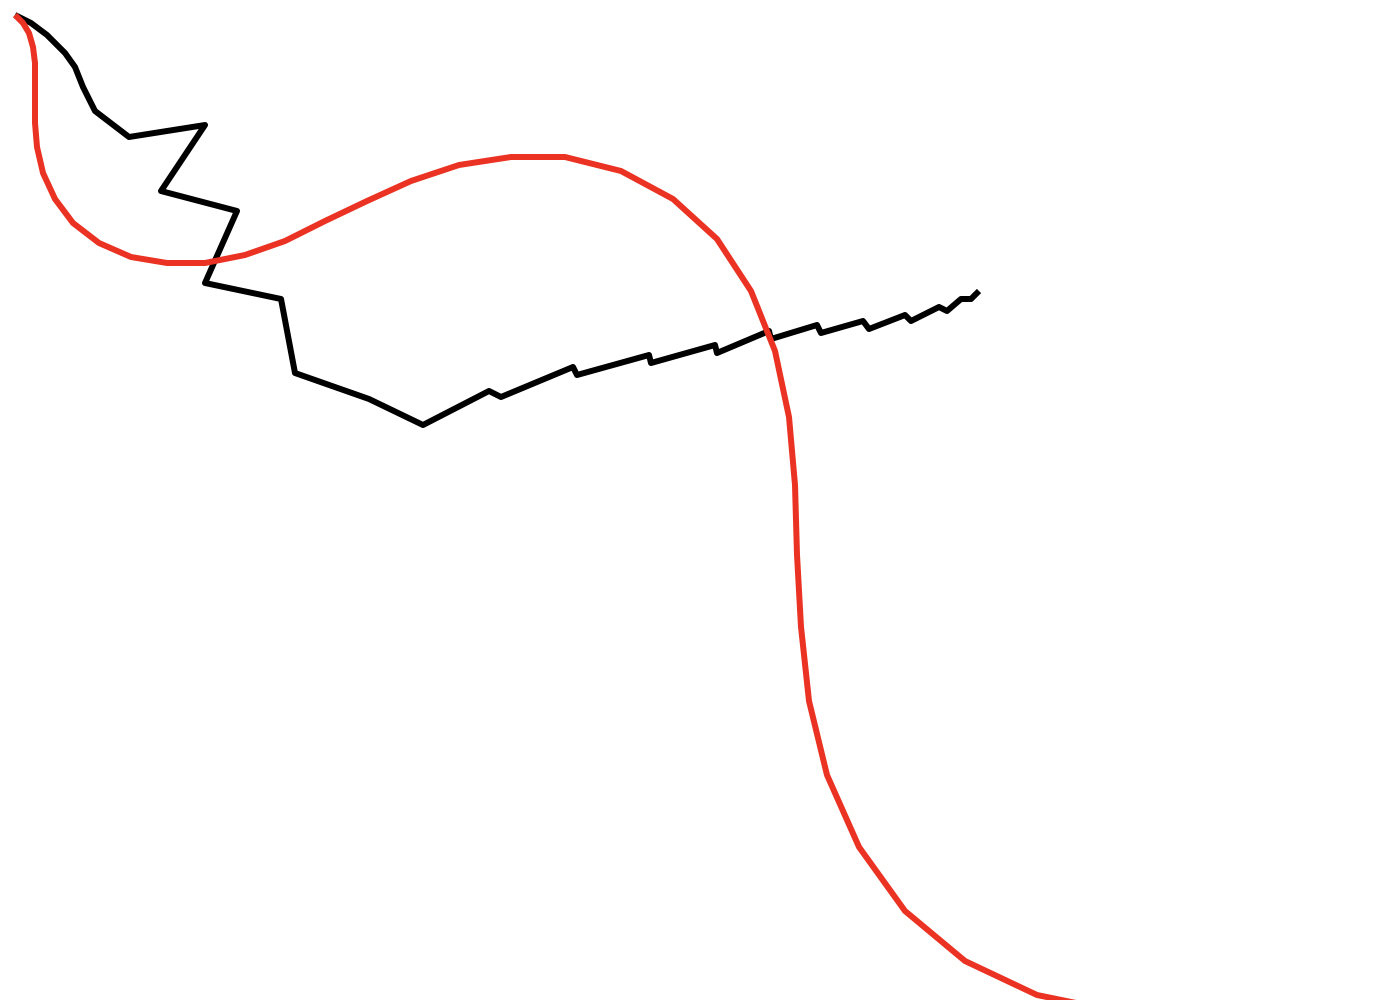
\includegraphics[width=\textwidth]{images/ddpg_results/envs_S3_S4_S5/S3_A2_R3_curve_A.png}
         \caption{$curve\_A$}
     \end{subfigure}
     \hfill
     \begin{subfigure}[b]{0.31\textwidth}
         \centering
         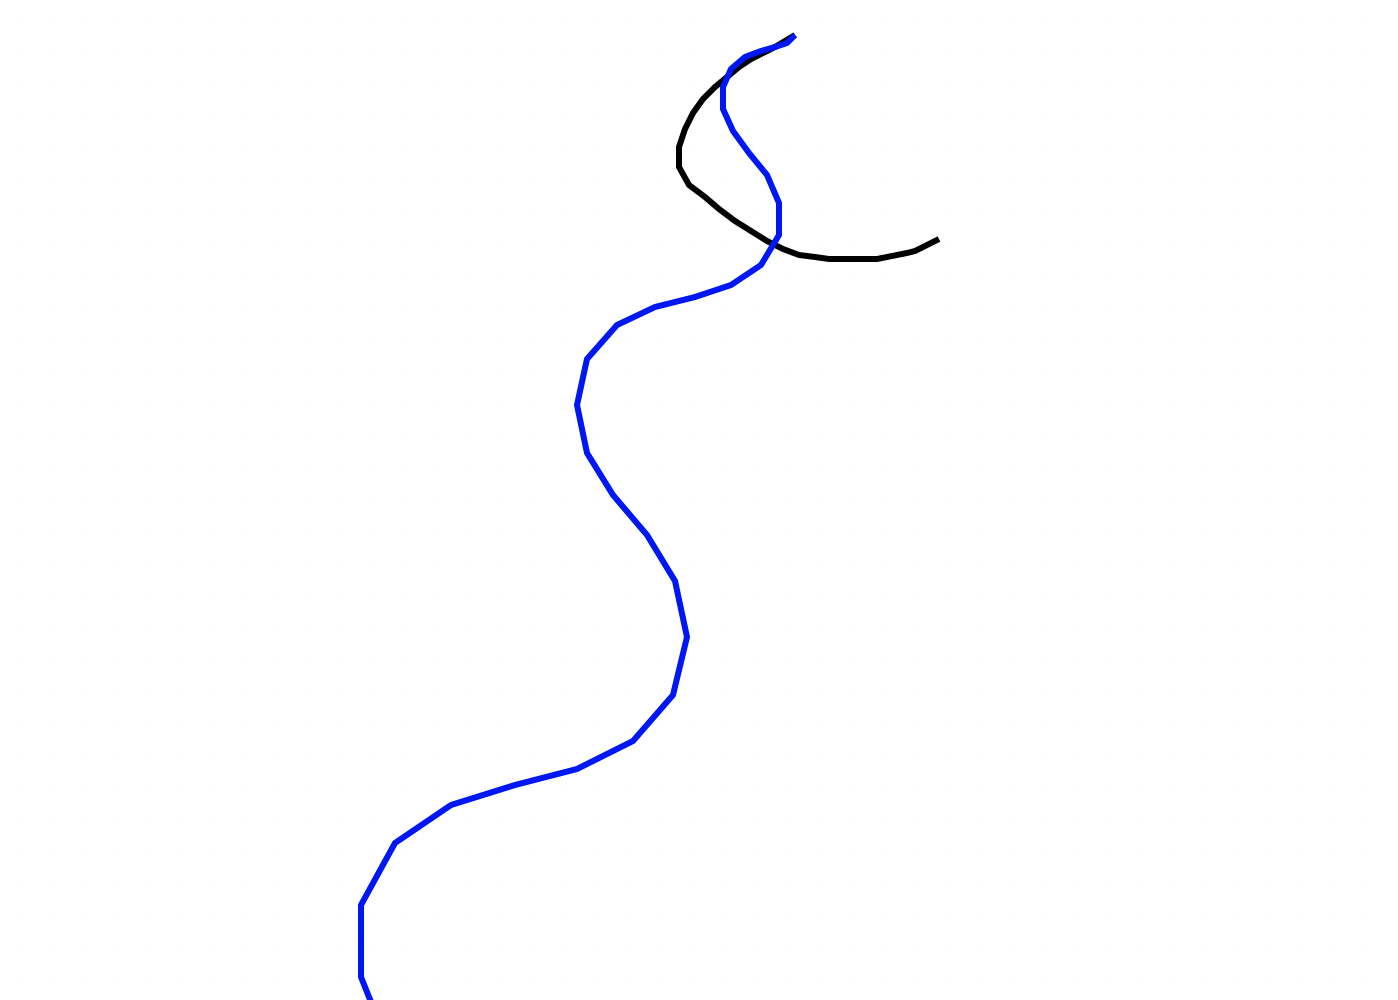
\includegraphics[width=\textwidth]{images/ddpg_results/envs_S3_S4_S5/S3_A2_R3_curve_B.png}
         \caption{$curve\_B$}
     \end{subfigure}
     \hfill
     \begin{subfigure}[b]{0.31\textwidth}
         \centering
         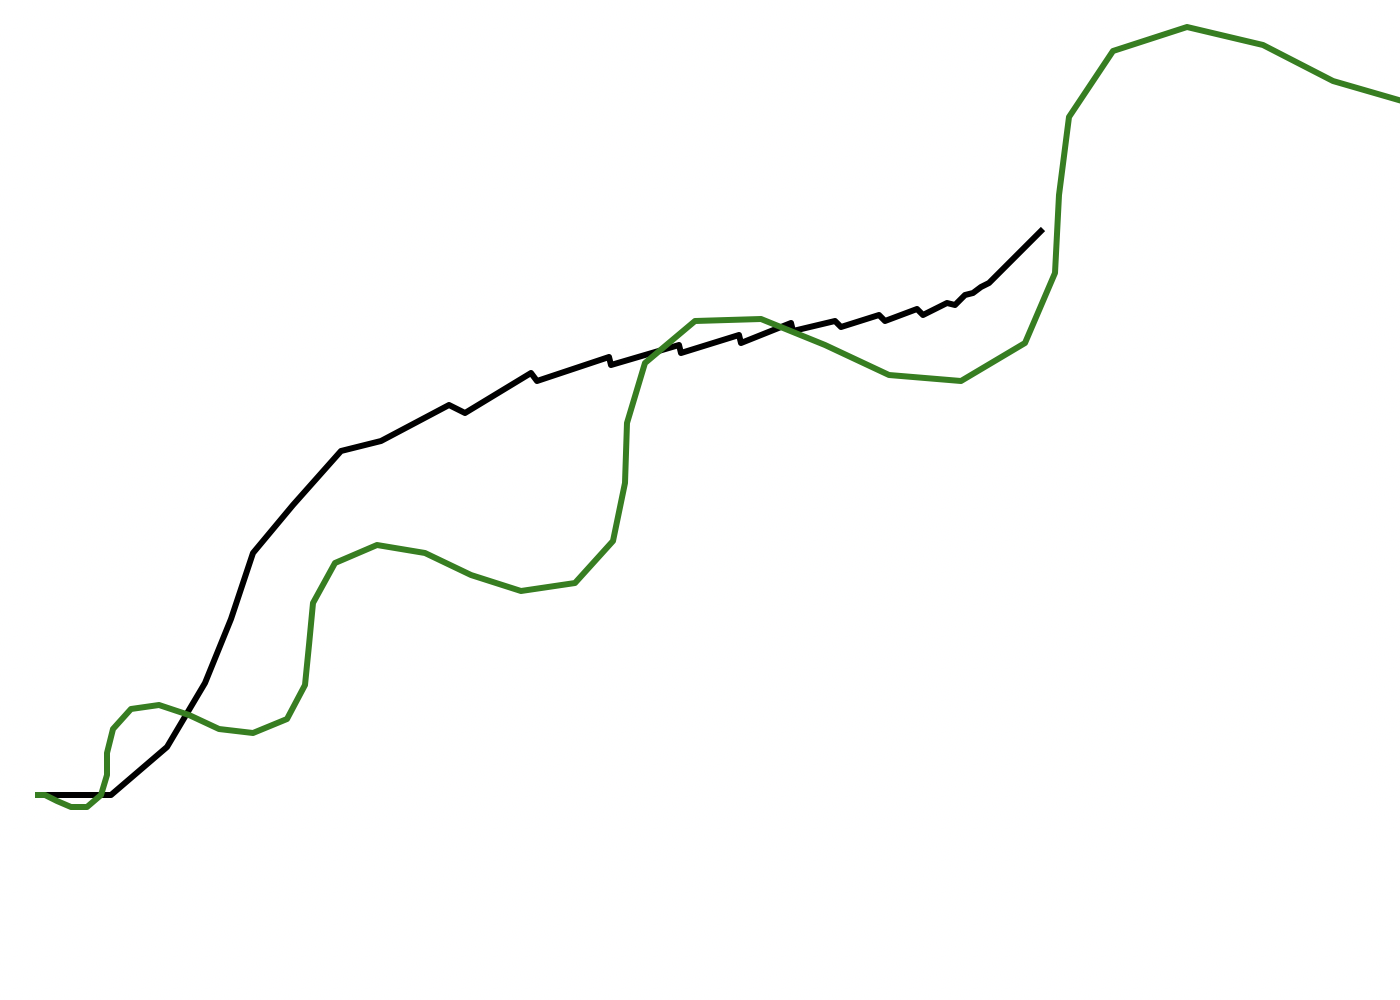
\includegraphics[width=\textwidth]{images/ddpg_results/envs_S3_S4_S5/S3_A2_R3_curve_C.png}
         \caption{$curve\_C$}
     \end{subfigure}
        \caption{$S3\_A2\_R3$ using $\sigma=0.15$ and a replay buffer size of $N=5\cdot 10^4$.}
        \label{fig:advCurves2}
\end{figure}


\begin{figure}[H]
     \centering
     \begin{subfigure}[b]{0.31\textwidth}
         \centering
         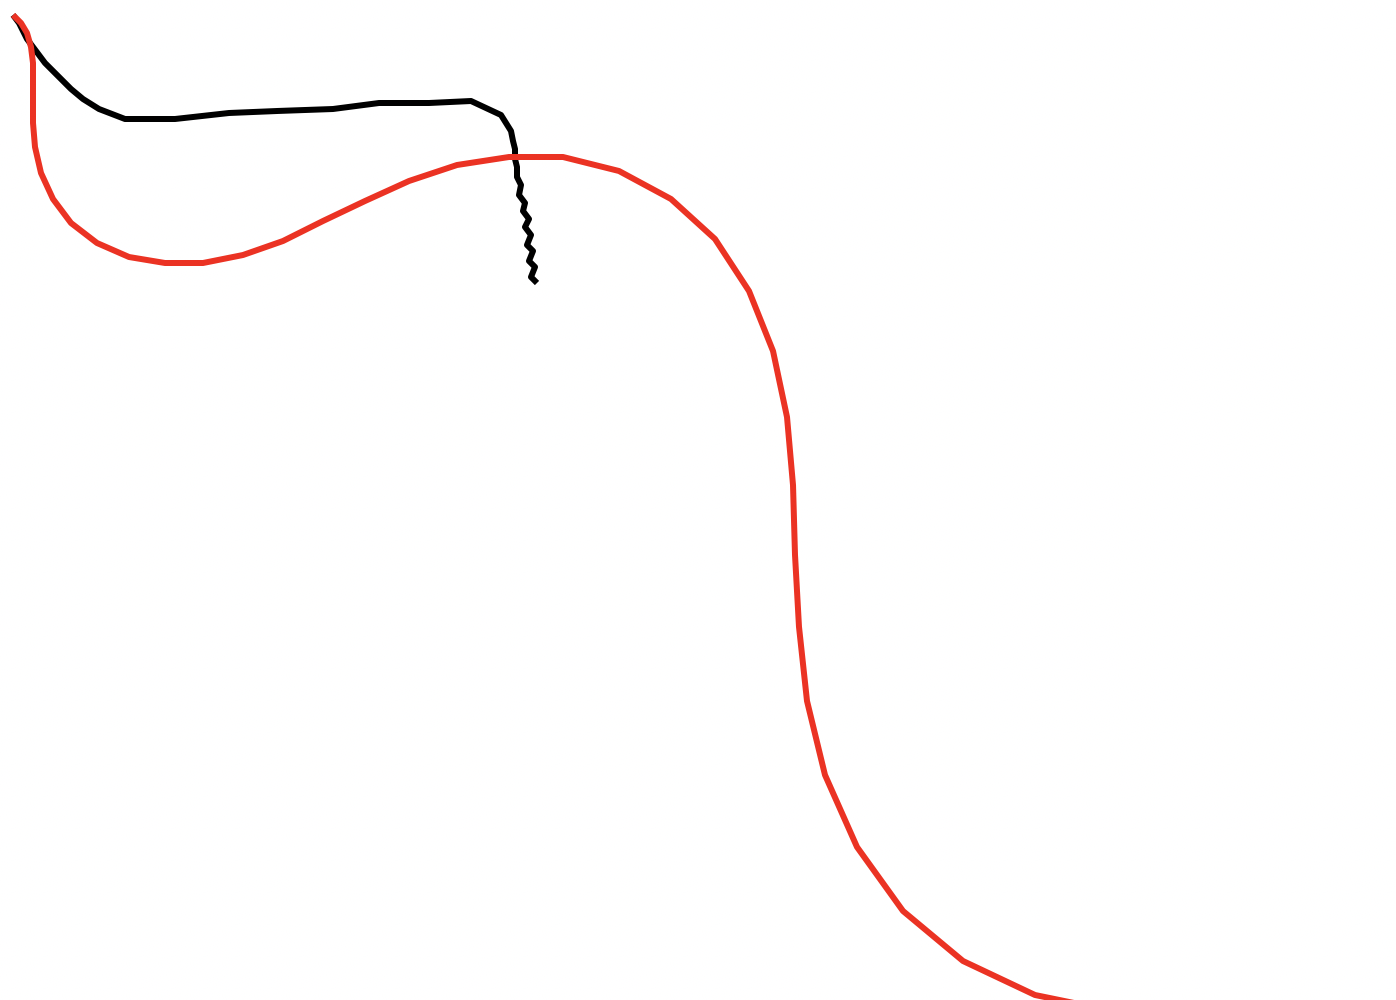
\includegraphics[width=\textwidth]{images/ddpg_results/envs_S3_S4_S5/S5_A2_R3_curve_A.png}
         \caption{$curve\_A$}
     \end{subfigure}
     \hfill
     \begin{subfigure}[b]{0.31\textwidth}
         \centering
         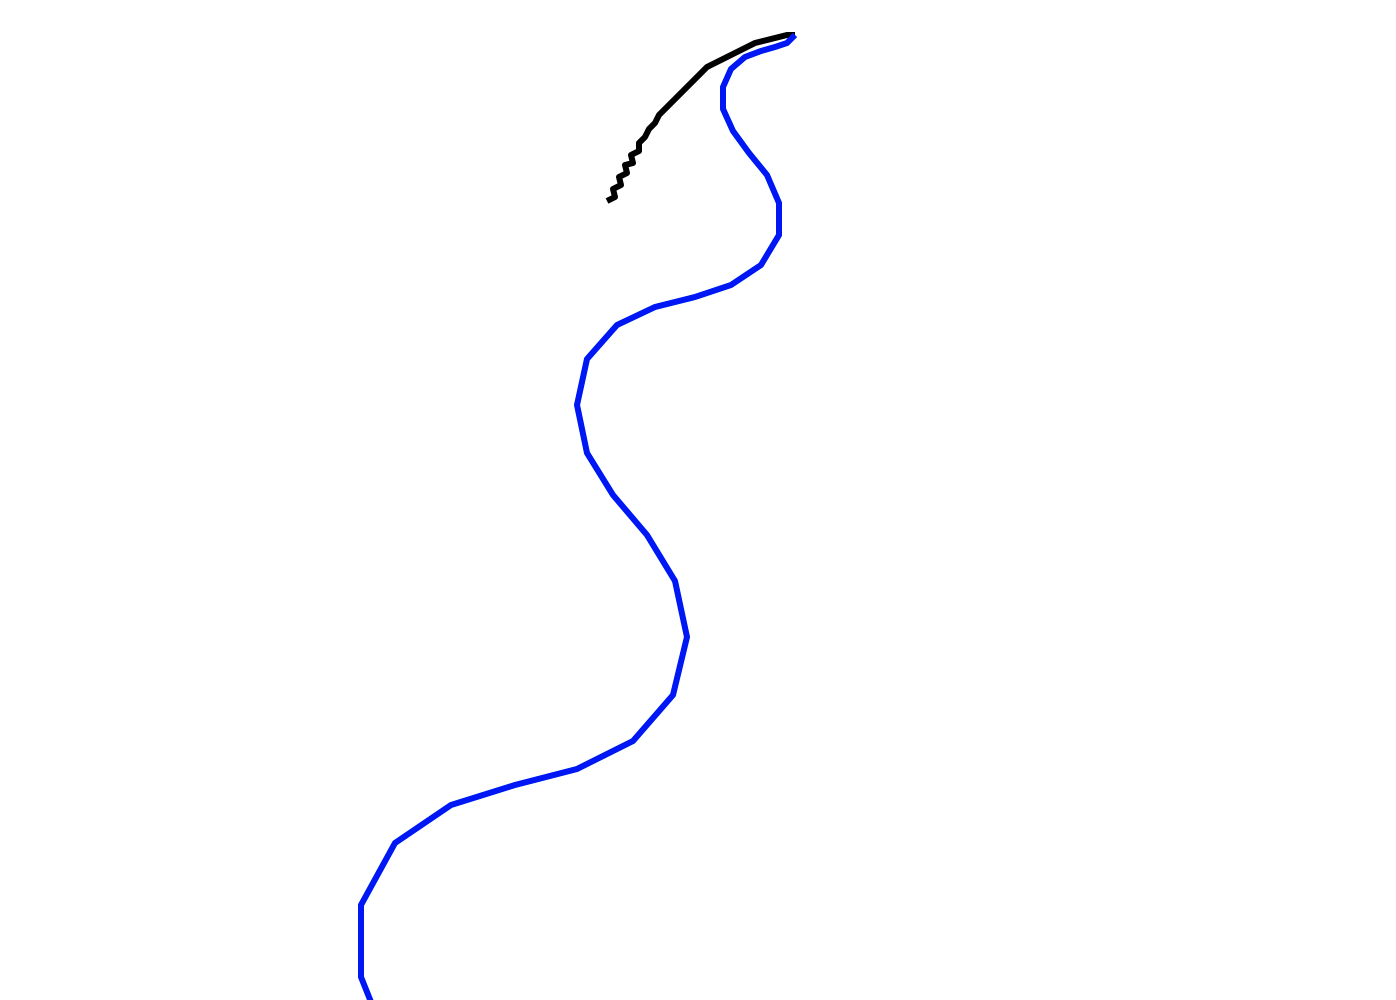
\includegraphics[width=\textwidth]{images/ddpg_results/envs_S3_S4_S5/S5_A2_R3_curve_B.png}
         \caption{$curve\_B$}
     \end{subfigure}
     \hfill
     \begin{subfigure}[b]{0.31\textwidth}
         \centering
         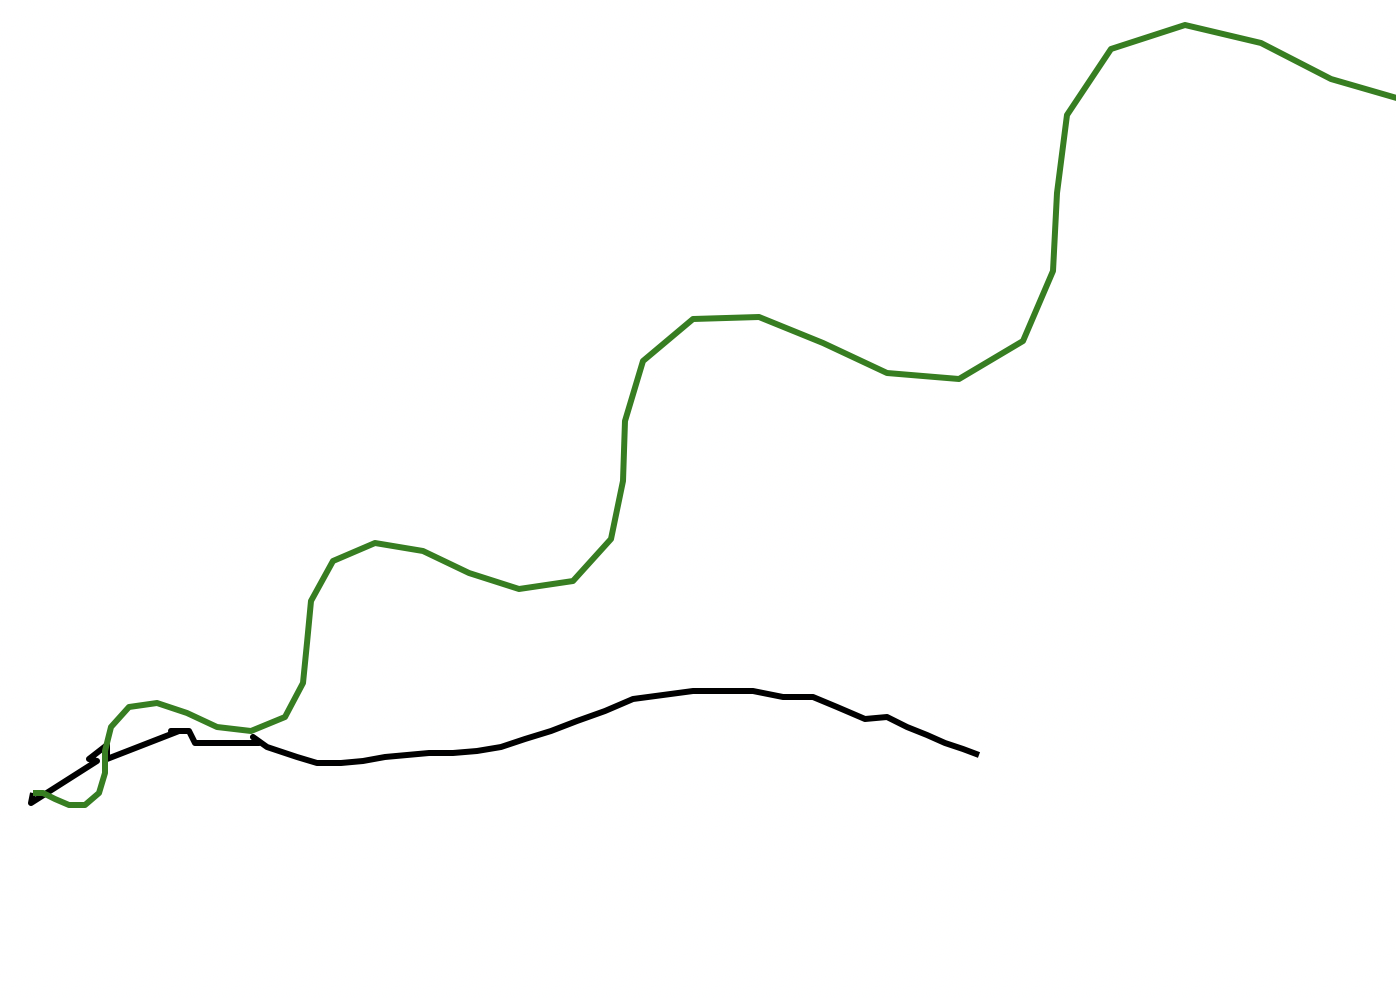
\includegraphics[width=\textwidth]{images/ddpg_results/envs_S3_S4_S5/S5_A2_R3_curve_C.png}
         \caption{$curve\_C$}
     \end{subfigure}
        \caption{$S5\_A2\_R3$ using $\sigma=0.15$ and a replay buffer size of $N=5\cdot 10^4$.}
        \label{fig:advCurves3}
\end{figure}
\newpage
The outcome illustrated in Fig. \ref{fig:advCurves1}, \ref{fig:advCurves2}, and \ref{fig:advCurves3} allow us to conclude that DDPG is not able to recover the direct optimal mapping in order to generate representative trajectories. No combination of replay buffer size, exploration magnitude, reward function, or applicable state representation shows respectable performance to the task. Still, there are some findings. One of them is the setting of $\sigma$, as a value above $0.3$ heavily impacts the performance negatively. Next, the replay buffer size shows no major effect on the outcomes, with $N=5 \cdot 10^4$ providing the best results. Besides that, the switch from identical learning rates for the actor and critic networks does indeed improve the performance of DDPG slightly (we include one experimental setup with the same learning rates in the appendix). A customization of the source code from the used library Stable-Baselines3 was necessary to allow for this usage of different learning rates. Moreover, the reward function $R3$ that sends out non-zero feedback at every time step provides better results than $R1$ and $R2$. Non-zero feedback is sent out every time step because the maximum distance for a positive reward is $100$, and during the training phase an episode is prematurely ended if the agent drifts apart from the GT more than $100$ pixels. Receiving feedback which directly translates to current distance to the GT, the agent has a supplementary indirect feature which helps to identify the current snapshot of the environment.
\par
With that in mind, we construct $S4$, which adds the current distance to the GT as a primary feature to the state space. During the initial experiment setup and the corresponding results shown in Tab. \ref{tab:resultsK3}, $S4$ yields the best performance, with $S4\_A2\_R3$ having an average distance of 80. In relation to the other state representations $S3$ and $S5$, this is a great improvement and thus gives a hint about why the other representations fail the task. But first, we visualize the proposed tracks by the fully trained agent in the upcoming Fig. \ref{fig:advCurves5}

\begin{figure}[H]
     \centering
         \includesvg[width=0.9\textwidth]{images/ddpg_results/envs_S3_S4_S5/ddpg_S4_A2_R3_K9.svg}
        \caption{Distances between the path proposed by the agent and the GT over time. $\sigma = 0.15$ and $N=5\cdot 10^4$.}
        \label{fig:advCurves4}
\end{figure}


\begin{figure}[H]
     \centering
     \begin{subfigure}[b]{0.31\textwidth}
         \centering
         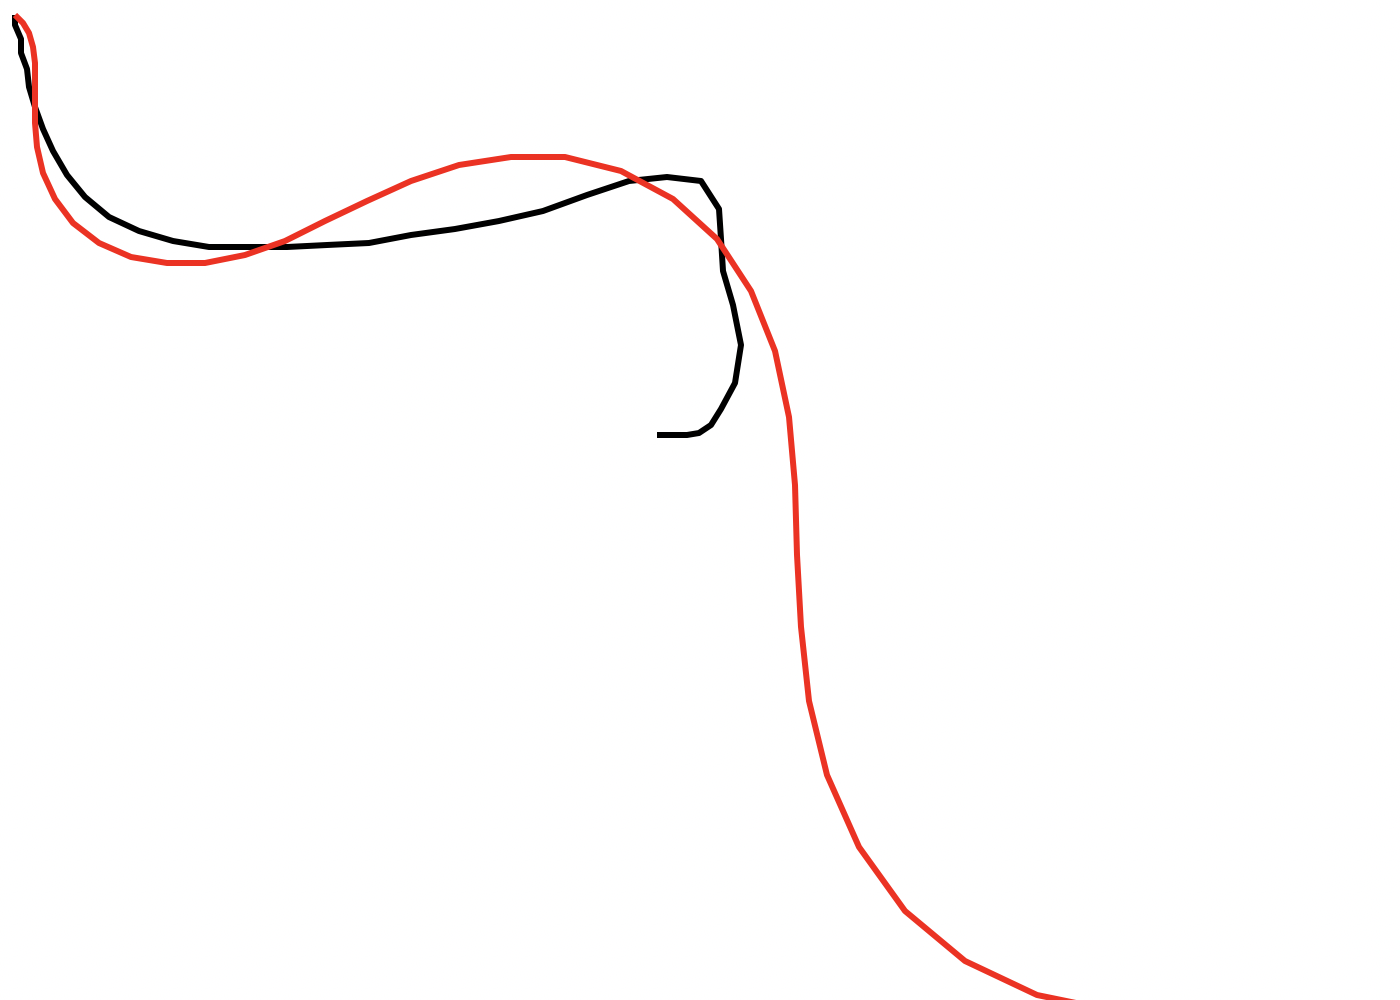
\includegraphics[width=\textwidth]{images/ddpg_results/envs_S3_S4_S5/S4_A2_R3_curve_A.png}
         \caption{$curve\_A$}
     \end{subfigure}
     \hfill
     \begin{subfigure}[b]{0.31\textwidth}
         \centering
         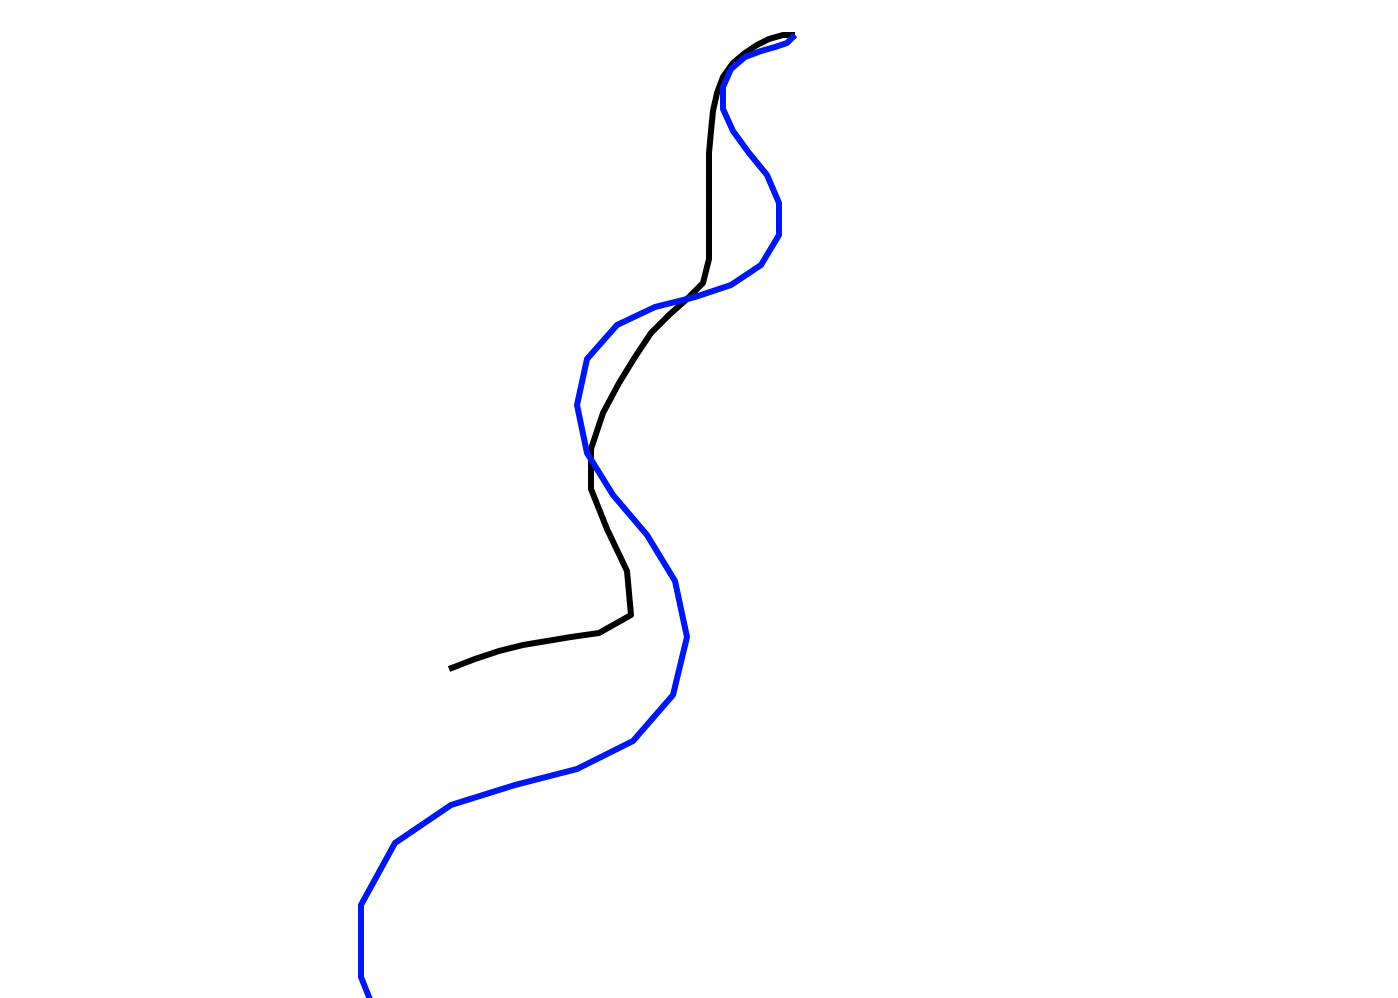
\includegraphics[width=\textwidth]{images/ddpg_results/envs_S3_S4_S5/S4_A2_R3_curve_B.png}
         \caption{$curve\_B$}
     \end{subfigure}
     \hfill
     \begin{subfigure}[b]{0.31\textwidth}
         \centering
         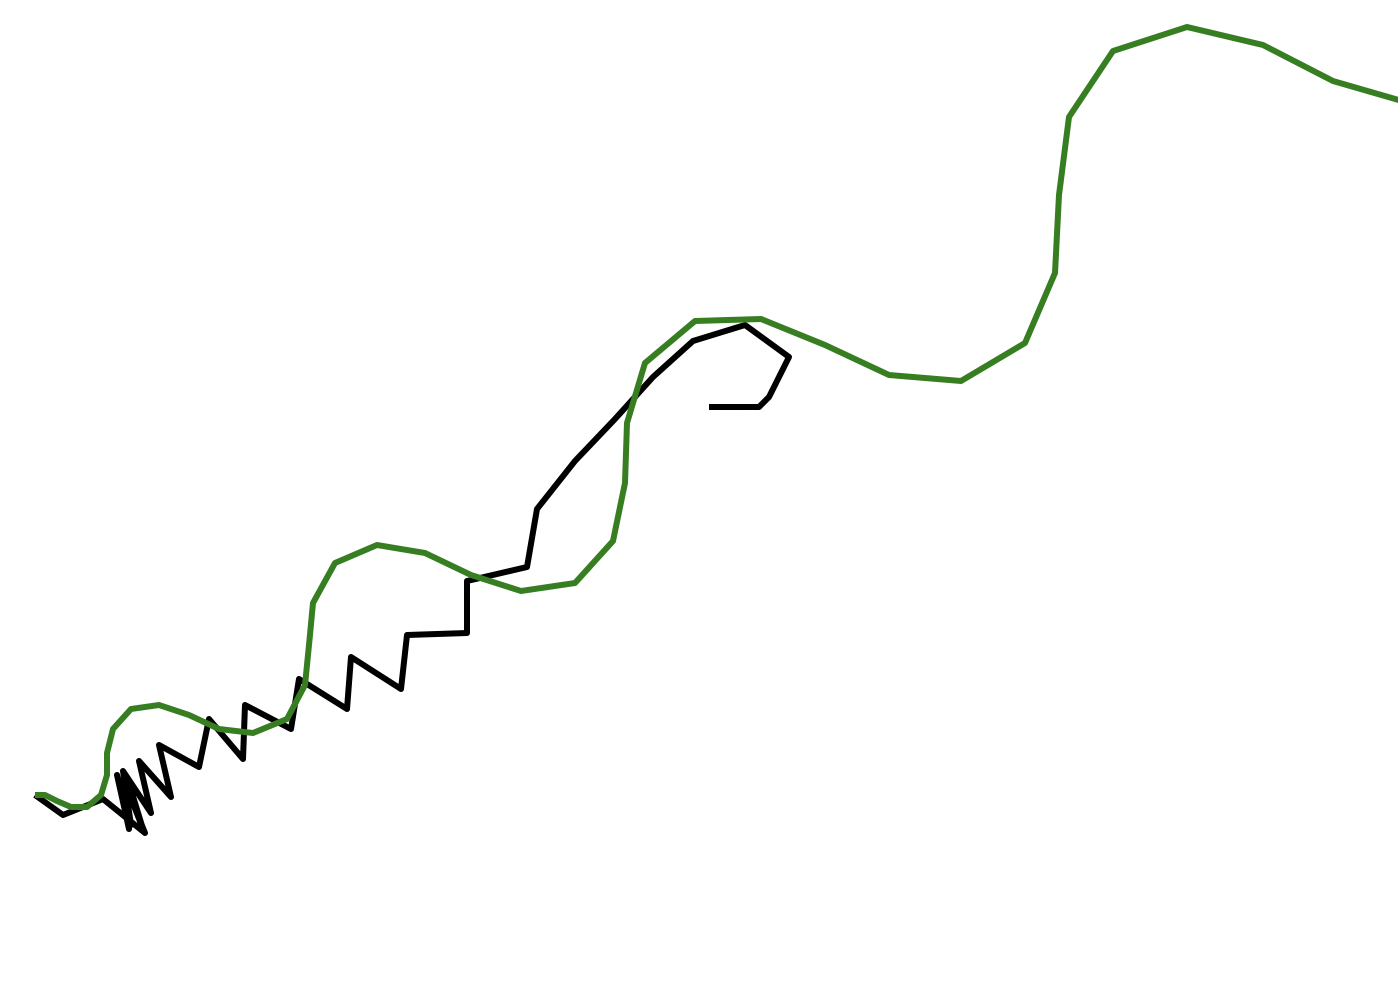
\includegraphics[width=\textwidth]{images/ddpg_results/envs_S3_S4_S5/S4_A2_R3_curve_C.png}
         \caption{$curve\_C$}
         \label{fig:a5c}
     \end{subfigure}
        \caption{$S4\_A2\_R3$ using $\sigma=0.05$ and a replay buffer size of $N=5\cdot 10^4$.}
        \label{fig:advCurves5}
\end{figure}

Although it has the best performance, $S4$ is still not able to fulfill the task on an acceptable level, which can be seen in Fig. \ref{fig:advCurves5}. However, in contrast to the previous visualized behaviors, the agent does not fluctuate in one area and is also able to generate paths that stay in the same region as the GT curve while heading in the same overall direction (best seen in Fig \ref{fig:a5c}).
\par
The reason behind the improved performance is the extended state space by a component that enhances the ability of the agent to separate between different snapshots of the environment during each episode. Previous state representations fail catastrophically because the replay buffer is filled with inconsistent feedback about state-action pairs that do seem to be the same in the eyes of the agent. For example, if the agent chooses a good action right at the beginning of an episode with fitting values of heading and speed while receiving $\{x, y, heading, speed\}$ as in $S3$, this transition gets saved into the replay buffer. This specific transition has a high positive reward because the next position of the agent is close to the GT. Assuming that the agent explores enough for the next time steps and ends up in the same state as the very first one. Even if the agent now chooses the perfect action again, the GT has already moved away, and in return the agent would be rewarded with a smaller value for this particular state-action pair than already saved in the replay buffer. As the episode continuous, the replay buffer gets overwhelmingly filled with transition tuples that indeed include the first state but with different reward values, which get smaller over time. Being filled with predominantly bad reward values for this specific state-action pair, the replay buffer is also responsible for the low Q-value assignment by the critic network because it is trained by randomly sampling the buffer.
\par
Adding the distance to the GT changes this behavior, as the agent is able to distinguish between different states during an episode and is also able to distinguish between different curves. Overall, we conclude that DDPG needs a very rich feature space that truly represents the environment at a certain time step and also allows the agent to choose actions to recover from bad states. In this instance, a high distance could potentially lead to a higher suggested value of speed. In the state representation of $S3$, there is no such thing as a recovery mechanism because the agent is unaware of the GT through the state space and only receives information about the GT position in the form of the reward signal. For direct policy learning, with the requirement of acting perfectly, as in conducting the perfect actions to follow the GT position at all time steps, DDPG seems to be the wrong approach. Especially, when the environment changes in the testing phase, because the GT is not present anymore and thus reducing the number of possible features.
\par
Besides the challenges of necessary feature engineering and state representation, we experience DDPG to be very susceptible to a variety of hyperparameters. From replay buffer sizes, exploration noise and learning rates, to the optimal reward function and different seeds, the performances of the separate runs varied significantly.